\section{亚线性复杂度PIR的基本构造}
由于我们选择基于现有的亚线性PIR方案构建可验证PIR~\cite{EC:CorKog20, C:LazPap23},对这些方案的认识是理解本文提出新方案的基础。我们从一个两服务器PIR方案开始,如图\ref{fig:CK20}所示,随后讨论如何修正该协议的局限性。该协议是一个离线-在线PIR方案,我们使用$\hintserver$ 与 $\queryserver$ 两个记号来区分协议中涉及到的两台服务器。稍后我们将会看到,这种记号是根据两台服务器的功能定义的:

\subsection{构造方案}

\noindent \textbf{离线阶段:}
\begin{itemize}
\item \textbf{Setup:} 客户端$\client$ 生成$\hintcount$ 组集合$\setkey_j, j\in[\hintcount]$。每个集合包含$\setsize$个在范围[$\dbsize$]内的随机索引。
\item \textbf{Hint:}$\client$将这些集合转发给$Hint$服务器$\hintserver$。$\hintserver$计算这些集合对应数据库中记录的和,表示为$\hint_j \coloneqq \sum_{k\in \setkey_j} \db_k, j \in [\hintcount]$。$\client$存储这些集合及其对应的和作为校验值。
\end{itemize}

\textbf{在线阶段:}
\begin{itemize}
\item \textbf{Query:}$\client$首先找出一个包含目标索引$\dbidx$的集合$\setkey_\hintidx$,并从该集合中去掉$\dbidx$,表示为$\queryquery \coloneqq \setkey_\hintidx \setminus \{\dbidx\}$。此外,$\client$生成一个包含索引$\dbidx$的新集合$\setkey'$,并将$\hintquery \coloneqq \setkey' \setminus \{\dbidx\}$。集合$\hintquery$被发送给$Hint$服务器$\hintserver$,而$\queryquery$被发送给$Query$服务器$\queryserver$。
\item \textbf{Answer:} 收到这些集合后,服务器分别为两个集合计算校验值,表示为$\queryanswer\coloneqq \sum_{j\in \queryquery}\db_j$和$\hintanswer\coloneqq \sum_{j\in \hintquery}\db_j$,并将这些校验值返回给$\client$。
\item \textbf{Reconstruct:}$\client$ 计算出所需的记录:$\db_\dbidx \coloneqq \hint_\hintidx - \queryanswer$。
\item \textbf{Refresh:}$\client$ 更新$Hint$: $\setkey_\hintidx \coloneqq \setkey'$,$\hint_\hintidx \coloneqq \hintanswer+\db_\dbidx$。
\end{itemize}


\subsection{基本构造的缺陷}
该协议的正确性是显而易见的。然而,该协议存在如下所列的三个关键问题:

\begin{enumerate}
\item \textbf{低效的集合查询:} 搜索包含查询索引$\dbidx$的合适集合$\setkey_t$的过程计算量较大。在我们的概念性协议中假设以明文形式存储集合,这需要客户端遍历所有集合才能找到合适的集合。尽管可以通过排序和二分查找进行优化,但它仍然会导致$O(\sqrt{\dbsize}\log \dbsize)$的客户端在线计算复杂度。
\item \textbf{低下的空间和通信效率:} 对客户端来说,以明文形式生成、存储和发送这些集合的效率低下,客户端完成协议时需要$O(\dbsize)$的存储和离线通信复杂度。大致上,为了确保在线阶段的正确性,客户端需要生成大约$\hintcount = O(\lambda\sqrt{\dbsize})$个集合,每个集合的大小为$\setsize = \sqrt{\dbsize}$。这会导致客户端存储和离线通信复杂度为$O(\lambda\dbsize)$。
\item \textbf{有缺陷的隐私性:} 集合$\queryquery$和$\hintquery$永远不包含查询的索引$\dbidx$。这泄露了大约$1/(\sqrt{\dbsize}\ln 2)$比特关于该索引的信息。
\end{enumerate}

\subsection{虚设查询及其引入的新问题}
在现有工作中,研究者已经提出了多种方法来解决上述问题。例如,TreePIR \cite{C:LazPap23} 利用了一种称为弱可打孔伪随机函数(Weakly Puncturable Pseudorandom Function)的原语,并引入了一种新的亚线性PIR构造。 Piano \cite{Piano} 提出了一个类似的算法,称为$PossibleParities$。然而,当涉及到可验证的PIR时,这些方案的适应性遇到了障碍。其原因本文将其总结为包含了“虚设查询”。

\begin{figure}
    \centering
    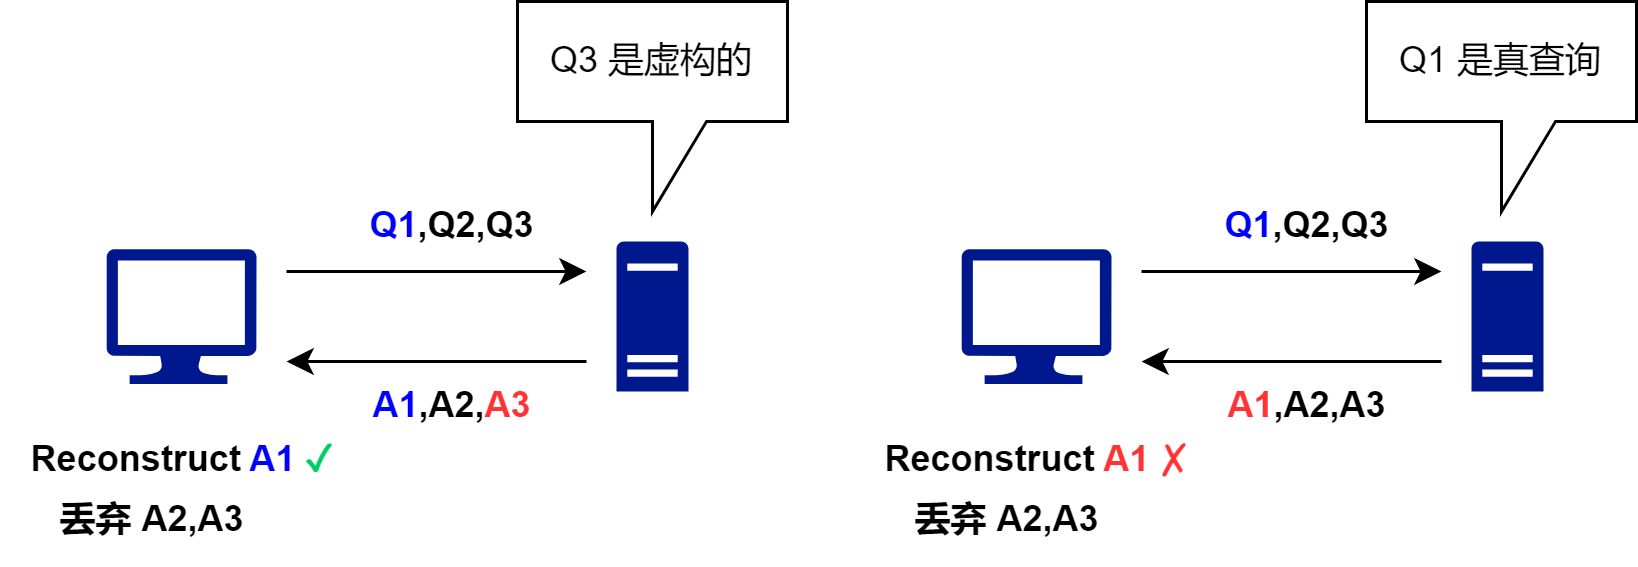
\includegraphics[width=1\linewidth]{figure/dummy.png}
    \caption{关于虚设查询的图示。客户端向服务器发送了3个查询,其中第一个查询是真实查询,另外两个是虚设查询。由于客户端只会拒绝对真实查询的错误答案,但会接受对虚设查询的错误答案,因此服务器可以通过操纵记录并从客户端的验证结果中推断出信息。}
    \label{fig:dummy}
\end{figure}

这些虚设查询是随机生成的假查询,目的是混淆真实查询。在这些方案中,客户端发送的单个查询会泄露关于查询索引$\dbidx$的信息给服务器。通过真实查询与虚设查询的组合,协议才得以隐藏了索引$\dbidx$。服务器会对虚设查询做出回应,但客户端会忽略对虚设查询的回应。CK20中的原始构造\cite{EC:CorKog20}并不遵循这一模式,因为他们方案中的查询都是有效查询,但并不总是查询所需的索引。换句话说,额外的查询并不是为了隐私,而是为了确保正确性。

在半诚实环境下,这些方案的隐私性依赖于服务器无法区分真实查询和虚设查询。然而,在可验证PIR的背景下,考虑到选择失败攻击,虚设查询会带来额外的麻烦。在验证过程中,客户端一般只能在真实查询的答案被篡改时拒绝服务器的响应。这是因为客户端没有在离线阶段获得这些虚设查询的校验信息,因此无法计算和验证虚设查询的答案。在这种情况下,服务器可以任意选择要篡改的答案,并且可以通过客户端的验证结果推断出被篡改的答案是否对应的是真实查询。这一漏洞使得恶意服务器有可能得知客户端正在查询的索引,从而导致我们无法在现有亚线性PIR方案中引入可验证性。图\ref{fig:dummy}展示了该问题的一个示例。除了隐私问题外,计算虚设查询的答案也增加了在线计算的成本。为了提高效率并应对选择失败攻击之间,我们的方案\textbf{消除了虚设查询}。

